%
% this file is encoded in utf-8
% v1.7
% do not change the content of this file
% unless the thesis layout rule is changed
% 無須修改本檔內容,除非校方修改了
% 封面、書名頁、中文摘要、英文摘要、誌謝、目錄、表目錄、圖目錄、符號說明
% 等頁之格式
% this file is encoded in utf-8
%v1.7

% make the line spacing in effect
\renewcommand{\baselinestretch}{\mybaselinestretch}
\large % it needs a font size changing command to be effective

% default variables definitions
% 注意!!此處只是預設值,不需更改此處
% 請更改 my_names.tex 內容
\newcommand\cTitle{論文題目}
\newcommand\eTitle{MY THESIS TITLE}
\newcommand\myCname{王鐵雄}
\newcommand\myEname{Aron Wang}
\newcommand\myStudentID{M9315048}
\newcommand\advisorCnameA{南宮明博士}
\newcommand\advisorEnameA{Dr.~Ming Nangong}
\newcommand\advisorCnameB{李斯坦博士}
\newcommand\advisorEnameB{Dr.~Stein Lee}
\newcommand\advisorCnameC{徐 石博士}
\newcommand\advisorEnameC{Dr.~Sean~Hsu}
\newcommand\univCname{國立台灣科技大學}
\newcommand\univEname{National Taiwan University of science and technology}
\newcommand\deptCname{光電工程研究所}
\newcommand\fulldeptEname{Graduate School of Electro-Optical Engineering}
\newcommand\deptEname{Electro-optical Engineering}
\newcommand\collEname{College of Engineering}
\newcommand\degreeCname{碩士}
\newcommand\degreeEname{Master of Science}
\newcommand\cYear{九十四}
\newcommand\cMonth{六}
\newcommand\cDay{十}
%\newcounter{eYear}
\newcommand\eYear{2006}
\newcommand\eMonth{June}
\newcommand\ePlace{Chungli, Taoyuan, Taiwan}


 % user's names; to replace those default variable definitions
%
% this file is encoded in utf-8
% v1.7
% 填入你的論文題目、姓名等資料
% 如果題目內有必須以數學模式表示的符號,請用 \mbox{} 包住數學模式,如下範例
% 如果中文名字是單名,與姓氏之間建議以全形空白填入,如下範例
% 英文名字中的稱謂,如 Prof. 以及 Dr.,其句點之後請以不斷行空白~代替一般空白,如下範例
% 如果你的指導教授沒有如預設的三位這麼多,則請把相對應的多餘教授的中文、英文名
%    的定義以空的大括號表示
%    如,\renewcommand\advisorCnameB{}
%          \renewcommand\advisorEnameB{}
%          \renewcommand\advisorCnameC{}
%          \renewcommand\advisorEnameC{}

% 論文題目 (中文)
\renewcommand\cTitle{%我的碩士論文題目 
巨量資料探勘框架:基於極限梯度提升之預測免費手機遊戲中潛在新進付費玩家
}

% 論文題目 (英文)
\renewcommand\eTitle{%My Thesis Title  
Big Data Mining Framework: Predicting Potential New Paying Player in Mobile Free-to-Play Games Based on Extreme Gradient Boosting
%My Thesis Title  \mbox{$\cal{H}_\infty$} and \mbox{Al$_x$Ga$_{1-x}$As}
}

% 我的姓名 (中文)
\renewcommand\myCname{廖宣瑋}

% 我的姓名 (英文)
\renewcommand\myEname{Hsuan-Wei Liao}

%我的學號
\renewcommand\myStudentID{M10715084}

% 指導教授A的姓名 (中文)
\renewcommand\advisorCnameA{戴文凱 博士}

% 指導教授A的姓名 (英文)
\renewcommand\advisorEnameA{Dr.~Wen-Kai Tai}

% 指導教授B的姓名 (中文)
\renewcommand\advisorCnameB{}

% 指導教授B的姓名 (英文)
\renewcommand\advisorEnameB{}

% 指導教授C的姓名 (中文)
\renewcommand\advisorCnameC{}

% 指導教授C的姓名 (英文)
\renewcommand\advisorEnameC{}

% 校名 (中文)
\renewcommand\univCname{國立臺灣科技大學}

% 校名 (英文)
%\renewcommand\univEname{National Taiwan University of science and technology}

% 系所名 (中文)
\renewcommand\deptCname{資~訊~工~程~系}

% 系所全名 (英文)
%\renewcommand\fulldeptEname{Graduate School of Electro-Optical Engineering}

% 系所短名 (英文, 用於書名頁學位名領域)
%\renewcommand\deptEname{Electro-Optical Engineering}

% 學院英文名 (如無,則以空的大括號表示)
%\renewcommand\collEname{College of Electrical and Communication Engineering}

% 學位名 (中文)
\renewcommand\degreeCname{碩士學位}

% 學位名 (英文)
%\renewcommand\degreeEname{Master of Science}

% 口試年份 (中文、民國)
\renewcommand\cYear{一\zero 〇\bai 九}

% 口試月份 (中文)
\renewcommand\cMonth{七} 

% 口試日期 (中文)
\renewcommand\cDay{二十一} 

% 口試年份 (阿拉伯數字、西元)
%\renewcommand\eYear{2009} 

% 口試月份 (英文)
%\renewcommand\eMonth{July}

% 學校所在地 (英文)
%\renewcommand\ePlace{Taipei, Taiwan}

%畢業級別;用於書背列印;若無此需要可忽略
\newcommand\GraduationClass{107}

%%%%%%%%%%%%%%%%%%%%%%
\newcommand\itsempty{}
%%%%%%%%%%%%%%%%%%%%%%%%%%%%%%%
%       ntust cover 封面
%%%%%%%%%%%%%%%%%%%%%%%%%%%%%%%
%
\begin{titlepage}
% no page number
% next page will be page 1

% aligned to the center of the page
\begin{center}
% font size (relative to 12 pt):
% \large (14pt) < \Large (18pt) < \LARGE (20pt) < \huge (24pt)< \Huge (24 pt)
%



\begin{figure}[htbp]
	\begin{minipage}[b]{5cm} 
		\raggedright
		
\includegraphics[width=1.1in]{frontpages/ntust_logo.eps}
		% \label{fig:ntust_logo}
	\end{minipage}% 
	\begin{minipage}[b]{0.5\textwidth} 
	\centering
	\makebox[3cm][c]{\Huge{\univCname}}\\  %顯示中文校名
	\vspace{0.5cm}
	\makebox[3cm][c]{\Huge{\deptCname}}\\ %顯示中文系所名
	\vspace{0.5cm}
	\end{minipage}%
\\ 
\rule{16cm}{3pt}
\end{figure}
%\hfill


\vspace{1cm}
\makebox[6cm][s]{\textbf{\Huge{\degreeCname 論文}}}\\ %顯示論文種類 (中文)
%\makebox[8cm][s]{\textbf{\Huge{\degreeCname 論文(初稿)}}}\\ %顯示論文種類 (中文)
\vspace{1cm}
%
% Set the line spacing to single for the titles (to compress the lines)
\renewcommand{\baselinestretch}{1}   %行距 1 倍
%\large % it needs a font size changing command to be effective
\Large{\cTitle}\\  % 中文題目
%
\vspace{1cm}
%
\Large{\eTitle}\\ %英文題目
\vspace{5cm}
% \makebox is a text box with specified width;
% option s: stretch
% use \makebox to make sure
% 「研究生:」 與「指導教授:」occupy the same width
\hspace{4.5cm} \makebox[3cm][s]{\Large{研 究 生:}}
\Large{\myCname}  % 顯示作者中文名
\hfill \makebox[1cm][s]{}\\
%
\vspace{0.3cm}
\hspace{4.5cm} \makebox[3cm][s]{\Large{學號:}}
\Large{\myStudentID}  %顯示指導教授A中文名
\hfill \makebox[1cm][s]{}\\
%
\vspace{1cm}
\hspace{4.5cm} \makebox[3cm][s]{\Large{指導教授:}}
\Large{\advisorCnameA}  %顯示指導教授A中文名
\hfill \makebox[1cm][s]{}\\
%
% 判斷是否有共同指導的教授 B
\ifx \advisorCnameB  \itsempty
\relax % 沒有 B 教授,所以不佔版面,不印任何空白
\else
% 共同指導的教授 B
\hspace{4.5cm} \makebox[3cm][s]{}
\Large{\advisorCnameB}  %顯示指導教授B中文名
\hfill \makebox[1cm][s]{}\\
\fi
%
% 判斷是否有共同指導的教授 C
\ifx \advisorCnameC  \itsempty
\relax % 沒有 C 教授,所以不佔版面,不印任何空白
\else
% 共同指導的教授 C
\hspace{4.5cm} \makebox[3cm][s]{}
\Large{\advisorCnameC}  %顯示指導教授C中文名
\hfill \makebox[1cm][s]{}\\
\fi
%
\vfill
\makebox[10cm][s]{\Large{中華民國\cYear 年\cMonth 月\cDay 日}}%
%
\end{center}
% Resume the line spacing to the desired setting
\renewcommand{\baselinestretch}{\mybaselinestretch}   %恢復原設定
% it needs a font size changing command to be effective
% restore the font size to normal
\normalsize
\end{titlepage}
%%%%%%%%%%%%%%

%% 從摘要到本文之前的部份以小寫羅馬數字印頁碼
% 但是從「書名頁」(但不印頁碼) 就開始計算
%\setcounter{page}{1}
\pagenumbering{Roman}
%\pagenumbering{arabic}
%%%%%%%%%%%%%%%%%%%%%%%%%%%%%%%
%       指導教授推薦書 
%%%%%%%%%%%%%%%%%%%%%%%%%%%%%%%
%
% insert the printed standard form when the thesis is ready to bind
% 在口試完成後,再將已簽名的推薦書放入以便裝訂
% create an entry in table of contents for 推薦書
% 反註解以下送出空白頁
% \newpage{\thispagestyle{empty}\addcontentsline{toc}{chapter}{\nameInnerCover}\mbox{}\clearpage}%
% \newpage

% 送出插入的文件
%
\includepdf[pages=-]{frontpages/reference_01.png} %推薦書
%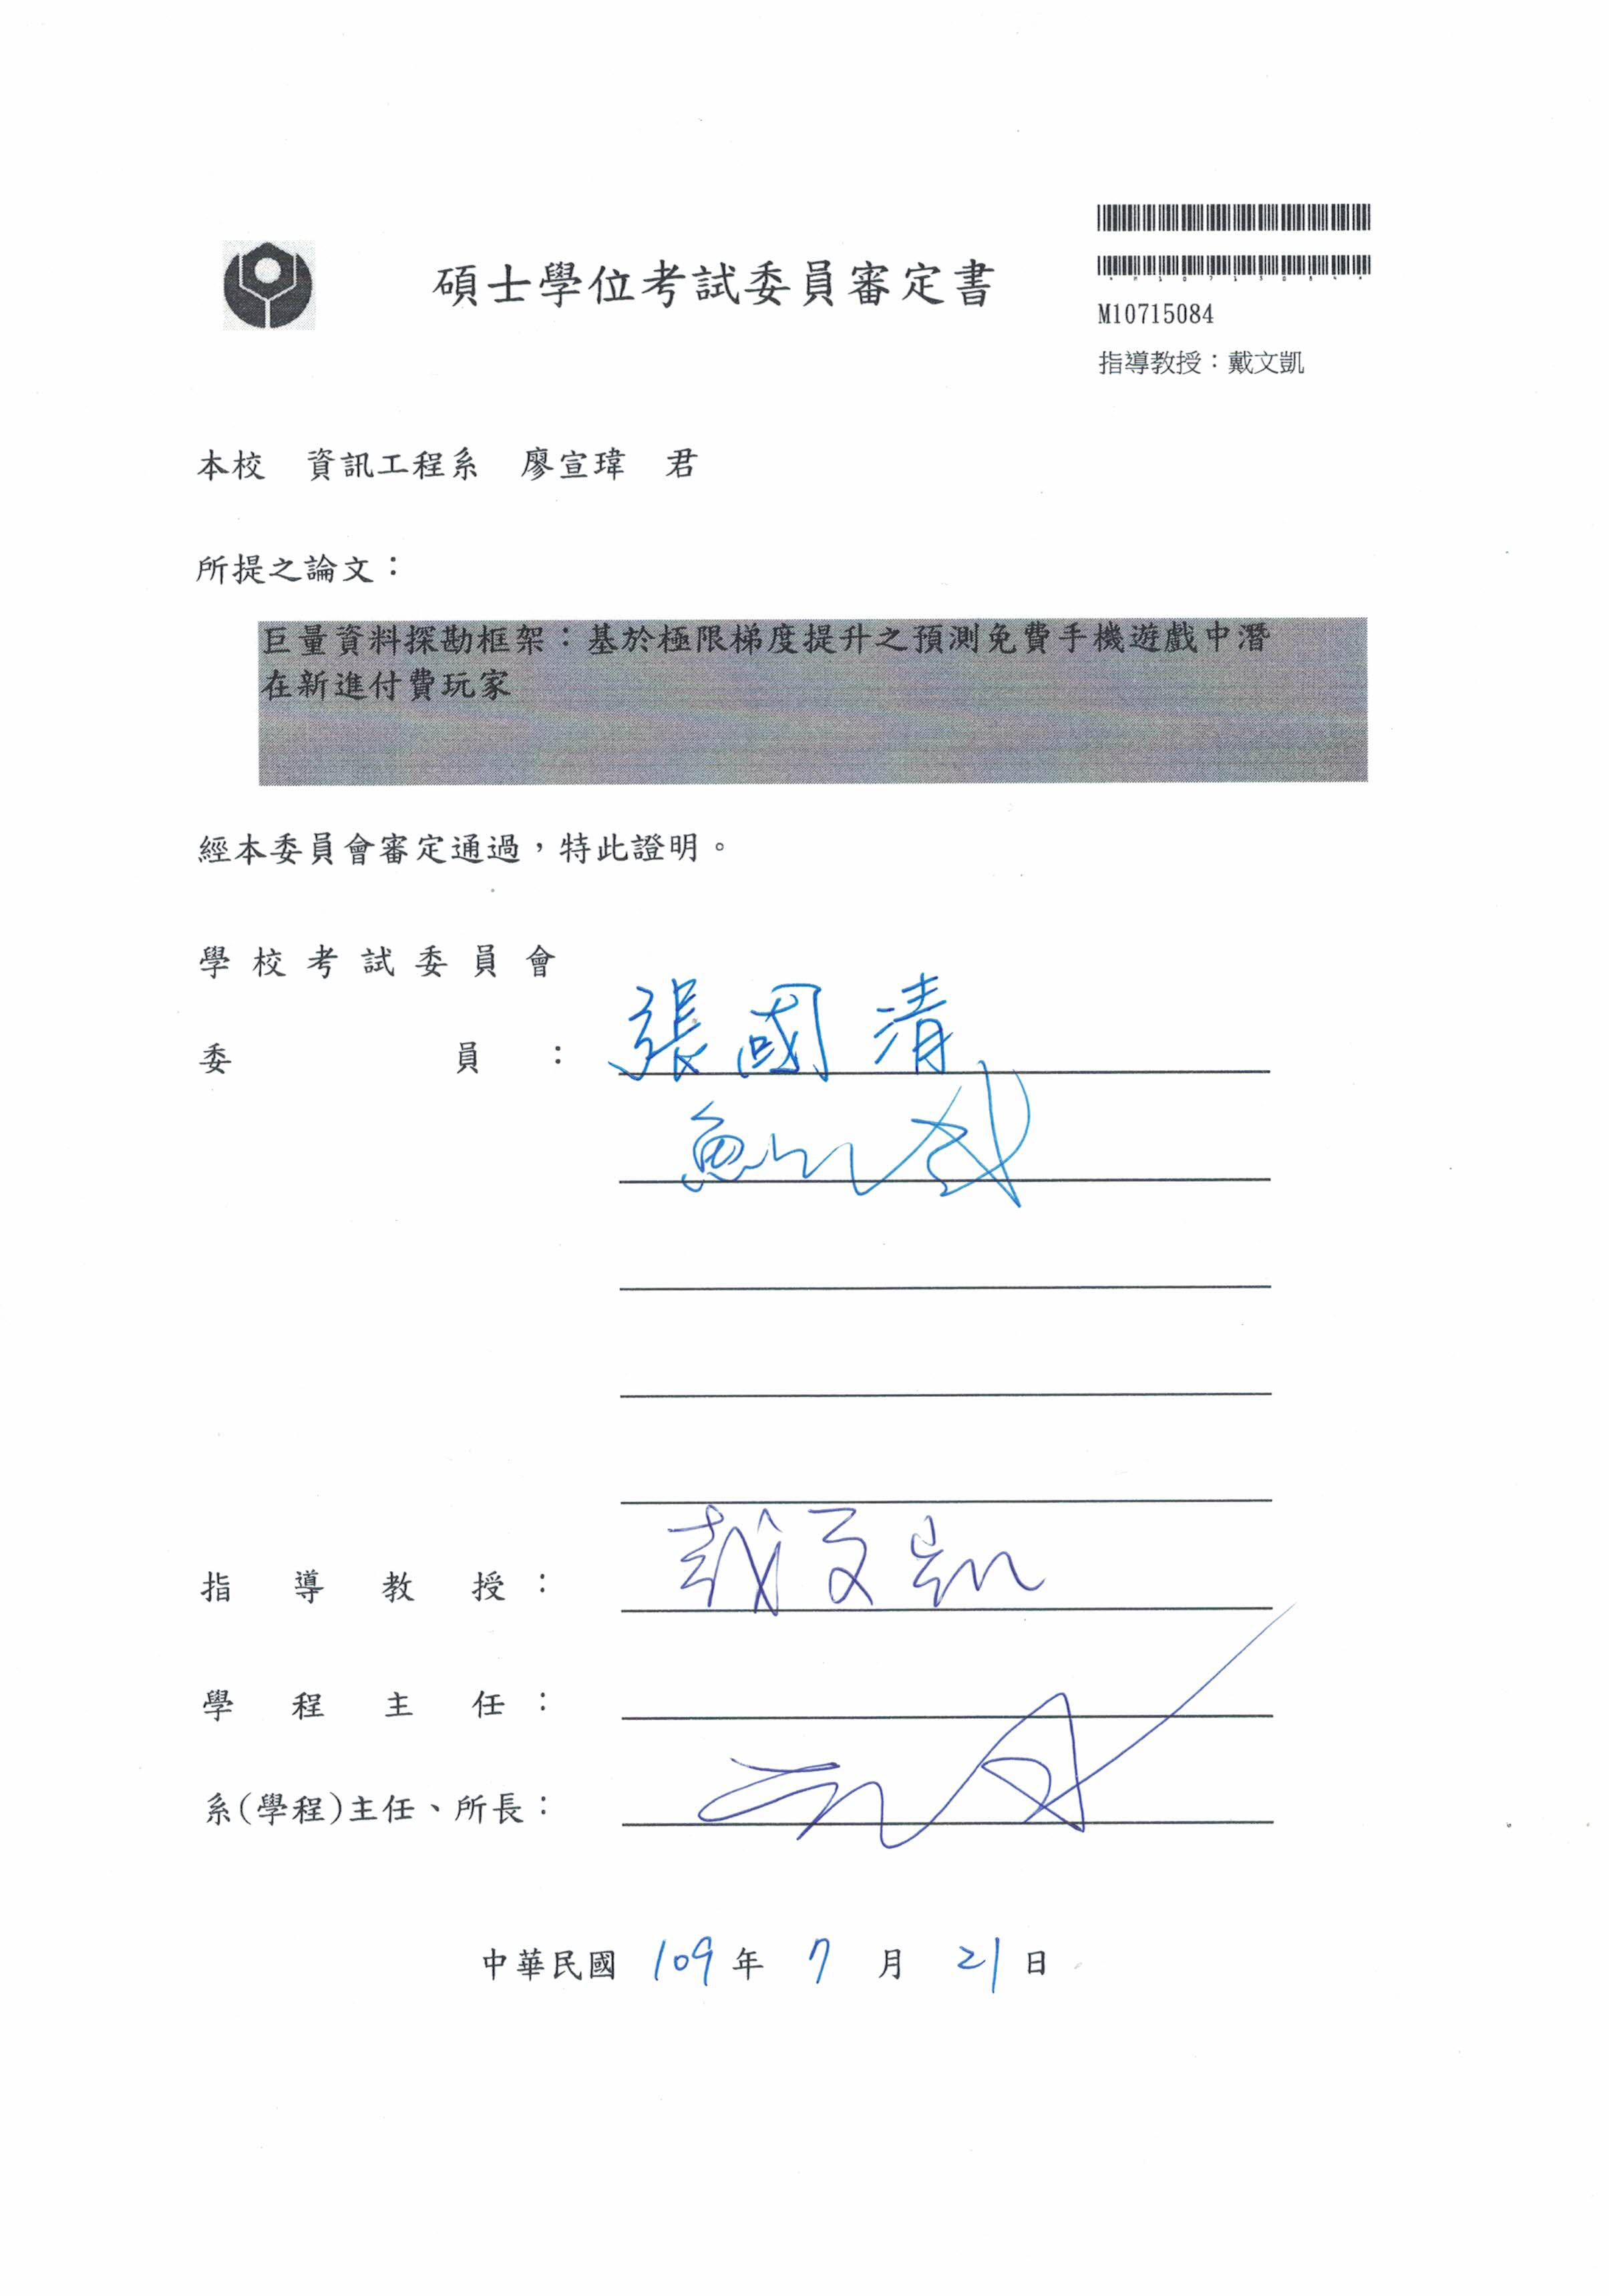
\includepdf[pages=-]{frontpages/reference_02.png} %審定書

% 判斷是否要浮水印?
\ifx\mywatermark\undefined 
  \thispagestyle{empty}  % 無頁碼、無 header (無浮水印)
\else
  \thispagestyle{EmptyWaterMarkPage} % 無頁碼、有浮水印
\fi

%%%%%%%%%%%%%%%%%%%%%%%%%%%%%%%%%%%%%%%%%%%%%%%%%%%%%%%%%%%%%%%
%%no page number
%% create an entry in table of contents for 書名頁
%\addcontentsline{toc}{chapter}{\nameInnerCover}
%
%
%% aligned to the center of the page
%\begin{center}
%% font size (relative to 12 pt):
%% \large (14pt) < \Large (18pt) < \LARGE (20pt) < \huge (24pt)< \Huge (24 pt)
%% Set the line spacing to single for the titles (to compress the lines)
%\renewcommand{\baselinestretch}{1}   %行距 1 倍
%% it needs a font size changing command to be effective
%%中文題目
%\Large{\cTitle}\\ %%%%%
%\vspace{1cm}
%% 英文題目
%\Large{\eTitle}\\ %%%%%
%%\vspace{1cm}
%\vfill
%% \makebox is a text box with specified width;
%% option s: stretch
%% use \makebox to make sure
%% 「研究生:」 與「指導教授:」occupy the same width
%\makebox[3cm][s]{\large{研 究 生:}}
%\makebox[3cm][l]{\large{\myCname}} %%%%%
%\hfill
%\makebox[2cm][s]{\large{Student: }}
%\makebox[5cm][l]{\large{\myEname}}\\ %%%%%
%%
%%\vspace{1cm}
%%
%\makebox[3cm][s]{\large{指導教授:}}
%\makebox[3cm][l]{\large{\advisorCnameA}} %%%%%
%\hfill
%\makebox[2cm][s]{\large{Advisor: }}
%\makebox[5cm][l]{\large{\advisorEnameA}}\\ %%%%%
%%
%% 判斷是否有共同指導的教授 B
%\ifx \advisorCnameB  \itsempty
%\relax % 沒有 B 教授,所以不佔版面,不印任何空白
%\else
%%共同指導的教授B
%\makebox[3cm][s]{}
%\makebox[3cm][l]{\large{\advisorCnameB}} %%%%%
%\hfill
%\makebox[2cm][s]{}
%\makebox[5cm][l]{\large{\advisorEnameB}}\\ %%%%%
%\fi
%%
%% 判斷是否有共同指導的教授 C
%\ifx \advisorCnameC  \itsempty
%\relax % 沒有 C 教授,所以不佔版面,不印任何空白
%\else
%%共同指導的教授C
%\makebox[3cm][s]{}
%\makebox[3cm][l]{\large{\advisorCnameC}} %%%%%
%\hfill
%\makebox[2cm][s]{}
%\makebox[5cm][l]{\large{\advisorEnameC}}\\ %%%%%
%\fi
%%
%% Resume the line spacing to the desired setting
%\renewcommand{\baselinestretch}{\mybaselinestretch}   %恢復原設定
%\large %it needs a font size changing command to be effective
%%
%\vfill
%\makebox[4cm][s]{\large{\univCname}}\\% 校名
%\makebox[6cm][s]{\large{\deptCname}}\\% 系所名
%\makebox[3cm][s]{\large{\degreeCname 論文}}\\% 學位名
%%
%%\vspace{1cm}
%\vfill
%\large{A Thesis}\\%
%\large{Submitted to }%
%%
%\large{\fulldeptEname}\\%系所全名 (英文)
%%
%%
%\ifx \collEname  \itsempty
%\relax % 沒有學院名 (英文),所以不佔版面,不印任何空白
%\else
%% 有學院名 (英文)
%\large{\collEname}\\% 學院名 (英文)
%\fi
%%
%\large{\univEname}\\%校名 (英文)
%%
%\large{in Partial Fulfillment of the Requirements}\\
%%
%\large{for the Degree of}\\
%%
%\large{\degreeEname}\\%學位名(英文)
%
%\large{in}\\
%%
%\large{\deptEname}\\%系所短名(英文;表明學位領域)
%%
%\large{\eMonth\ \eYear}\\%月、年 (英文)
%%
%\large{\ePlace}% 學校所在地 (英文)
%\vfill
%\large{中華民國}%
%\large{\cYear}% %%%%%
%\large{年}%
%\large{\cMonth}% %%%%%
%\large{月}\\
%\end{center}
%% restore the font size to normal
%\normalsize
%\clearpage


%%%%%%%%%%%%%%%%%%%%%%%%%%%%%%%%%%%%%%%%%%%%%%%%%%%%%%%%%%%%%%%%%%%%%
%%%%%%%%%%%%%%%%%%%%%%%%%%%%%%%
%       論文口試委員審定書 (計頁碼,但不印頁碼) 
%%%%%%%%%%%%%%%%%%%%%%%%%%%%%%%
%
% insert the printed standard form when the thesis is ready to bind
% 在口試完成後,再將已簽名的審定書放入以便裝訂
% create an entry in table of contents for 審定書
% 目前送出空白頁

%\newpage{\thispagestyle{empty}\addcontentsline{toc}{chapter}{\nameCommitteeForm}\mbox{}\clearpage}%


%%%%%%%%%%%%%%%%%%%%%%%%%%%%%%%
%       中文摘要 
%%%%%%%%%%%%%%%%%%%%%%%%%%%%%%%
%
%%%\newpage
%%%\thispagestyle{plain}  % 無 header,但在浮水印模式下會有浮水印
% create an entry in table of contents for 中文摘要
%%%\phantomsection
%%%\addcontentsline{toc}{chapter}{\nameCabstract}

% aligned to the center of the page
%%%\begin{center}
%%%	\makebox[5cm][s]{\LARGE{中文摘要}}\\
%%%\end{center}
% Resume the line spacing to the desired setting
%%%\renewcommand{\baselinestretch}{\mybaselinestretch}
%it needs a font size changing command to be effective
% restore the font size to normal
\normalsize
%%%%%%%%%%%%%
%%%\noindent
%%%目前市面上之手機遊戲多以免費遊玩商業模式(Free-to-Play, F2P)為主,使得遊戲內購買( In-App Purchase, IAP)顯得越來越重要,已然成為遊戲開發商營運之重點,為了能夠推出成功吸引各式玩家的精準行銷,需要資料分析團隊針對付費玩家進行研究,並且希望能夠在新進玩家族群中,成功預測出潛在付費玩家,以利提升IAP的意願,因此,如何在付費玩家資料中,有效探勘出資料特徵並透過機器學習進行預測,則為此次研究的目標。

本論文對此議題提出一巨量資料探勘框架,將需先將資料進行前處理以及預測前之資料分析,隨後訓練機器學習與其最佳化處理,最後再依預測之結果導入資料特徵重要性分析之中,完成整體預測與分析之工作,此框架將由四大階段組成: (1) 資料前處理階段、(2) 資料分析階段、(3) 機器學習階段及(4) 預測結果分析階段。

根據實驗結果,藉由我們提出的巨量資料探勘框架,利用無價值玩家觀察期清理了無價值的資料,並藉由付費玩家定義期準備了付費玩家與非付費玩家目標值,利用資料特徵探勘期探勘出了有價值的玩家遊戲行為軌跡。透過探索性資料分析(Exploratory Data Analysis, EDA)找出不合理資料特徵與高資訊量資料特徵,推測出有價值的資料特徵。能夠經由學習模型之預測,預測出潛在之新進付費玩家,並依其預測結果,分析資料特徵重要性,了解到玩家消費原因與遊戲之連動性。整體來說,該框架將能使得預測付費玩家之時間成本與人力成本有效降低,並得到對於行銷有利的資訊。

關鍵字:付費預測、免費遊玩遊戲、巨量資料、資料探勘、機器學習、極限梯度提升
%%%\newpage

%%%%%%%%%%%%%%%%%%%%%%%%%%%%%%%
%       英文摘要 
%%%%%%%%%%%%%%%%%%%%%%%%%%%%%%%
%
%%%\thispagestyle{plain}  % 無 header,但在浮水印模式下會有浮水印
% create an entry in table of contents for 英文摘要
%%%\phantomsection
%%%\addcontentsline{toc}{chapter}{\nameEabstract}
% aligned to the center of the page
%%%\begin{center}
	% \renewcommand{\baselinestretch}{1}   %行距 1 倍
%%%	\makebox[\width][s]{\LARGE{ABSTRACT}}\\
%%%\end{center}
% Resume the line spacing the desired setting
%%%\renewcommand{\baselinestretch}{\mybaselinestretch}   %恢復原設定
%\large %it needs a font size changing command to be effective
% restore the font size to normal
%%%\normalsize
%%%%%%%%%%%%%
%%%
In recent years, most mobile game developers focus on free-to-play (F2P) games. However, it is extremely difficult for F2P games to define whether players are churning, which makes game operators hard to retain players. In addition, new players have a higher churn rate. Therefore, if operators can accurately predict the new players that may churn, they can immediately adopt a retention strategy to lost players, looking forward that this will increase the retention rate of new players and thus effectively increase revenue.

This thesis proposes a machine learning framework for this topic, which is composed of five major stages: (1) pre-processing stage, (2) analysis stage, (3) machine learning stage, (4) feature extraction analysis stage and (5) businese application analysis stage. To be specific, the framework will need to process the data and data analysis before prediction, and train the model via machine learning algorithm, then analyze important features with the prediction results. Finally, by using surrogate model, the framework will be able to find out the patterns of player churn.

Keywords: New Player, Churn Prediction, Free-to-Play, Machine Learning

%%%%%%%%%%%%%%%%%%%%%%%%%%%%%%%
%       誌謝 
%%%%%%%%%%%%%%%%%%%%%%%%%%%%%%%
%
% Acknowledgment
%%%\newpage
% \chapter*{\protect\makebox[5cm][s]{\nameAckn}} %\makebox{} is fragile; need protect
%%%\phantomsection
%%%\addcontentsline{toc}{chapter}{\nameAckn}
%%%\begin{center}
%%%	\makebox[5cm][s]{\LARGE{誌謝}}\\
%%%\end{center}
%%%
非常感謝指導教授戴文凱博士,在我的碩士生涯中給予我許多的指導,在討論研究時,老師都會適時地指出不足之處;在撰寫論文時,老師也都會幫忙審查,並時常會叮嚀我注意小細節,讓我能順利的完成本論文,再次感謝老師的教導與協助。

另外,特別感謝張國清博士,時常在我研究時給予我建議,並指正我錯誤的部分,讓我的實驗結果有不錯的表現;在我於公司實習時,也都會額外花時間教學與照顧,讓我額外學到許多與產業應用相關的部份,再次感謝張博士的鼎力相助。

最後感謝一路上陪伴我求學的家人們,在我感到壓力時,能給我許多溫暖與依靠;在我遇到困難時,能給我極大的鼓勵與支持,讓我能夠持續堅持下去,且不顧一切地繼續往前走,真的很感謝我的家人們。

%%%%%%%%%%%%%%%%%%%%%%%%%%%%%%%
%       目錄 
%%%%%%%%%%%%%%%%%%%%%%%%%%%%%%%
%
% Table of contents
%%%\newpage
%%%\renewcommand{\contentsname}{\protect\makebox[5cm][s]{\nameToc}}
%\makebox{} is fragile; need protect
%%%\phantomsection
%%%\addcontentsline{toc}{chapter}{\nameToc}
%%%\tableofcontents

%%%%%%%%%%%%%%%%%%%%%%%%%%%%%%%
%       圖目錄 
%%%%%%%%%%%%%%%%%%%%%%%%%%%%%%%
%
% List of Figures
%%%\newcommand{\loflabel}{圖}
%%%\newpage
%%%\renewcommand{\numberline}[1]{\loflabel~#1\hspace*{1em}}
%%%\renewcommand{\listfigurename}{\protect\makebox[5cm][s]{\nameTof}}
%\makebox{} is fragile; need protect
%%%\phantomsection
%%%\addcontentsline{toc}{chapter}{\nameTof}
%%%\listoffigures

%%%%%%%%%%%%%%%%%%%%%%%%%%%%%%%
%       表目錄 
%%%%%%%%%%%%%%%%%%%%%%%%%%%%%%%
%
% List of Tables
%%%\newcommand{\lotlabel}{表}
%%%\newpage
%%%\renewcommand{\numberline}[1]{\lotlabel~#1\hspace*{1em}}
%%%\renewcommand{\listtablename}{\protect\makebox[5cm][s]{\nameLot}}
%\makebox{} is fragile; need protect
%%%\phantomsection
%%%\addcontentsline{toc}{chapter}{\nameLot}
%%%\listoftables

%%%%%%%%%%%%%%%%%%%%%%%%%%%%%%%
%       演算法目錄 
%%%%%%%%%%%%%%%%%%%%%%%%%%%%%%%
%
% List of Figures
%\newpage
%\renewcommand{\listalgorithmname}{\protect\makebox[5cm][s]{\nameToa}}
%\makebox{} is fragile; need protect
%\addcontentsline{toc}{chapter}{\nameToa}
%\listofalgorithms


%%%%%%%%%%%%%%%%%%%%%%%%%%%%%%%
%       符號說明 
%%%%%%%%%%%%%%%%%%%%%%%%%%%%%%%
%
% Symbol list
% define new environment, based on standard description environment
% adapted from p.60~64, <<The LaTeX Companion>>, 1994, ISBN 0-201-54199-8
%%%\newcommand{\SymEntryLabel}[1]%
%%%{\makebox[3cm][l]{#1}}

%%%\newenvironment{SymEntry}
%%%  {\begin{list}{}%
%%%      {\renewcommand{\makelabel}{\SymEntryLabel}%
%%%       \setlength{\labelwidth}{3cm}%
%%%       \setlength{\leftmargin}{\labelwidth}%
%%%       }%
%%%  }%
%%%  {\end{list}}
%
%%%\newpage
%%%\phantomsection
%%%\chapter*{\protect\makebox[5cm][s]{\nameSlist}} %\makebox{} is fragile; need protect
%%%\addcontentsline{toc}{chapter}{\nameSlist}
%%%%
% this file is encoded in utf-8
% v1.7
% 各符號以 \item[] 包住,然後接著寫說明
% 如果符號是數學符號,應以數學模式表示,以取得正確的字體
% 如果符號本身帶有方括號,則此符號可以用大括號 {} 包住保護
\begin{SymEntry}

    \item[$O$]
    觀察期天數

    \item[$R$]
    挽留期天數
    
    \item[$P$]
    表現期天數
    
    \item[$class\ 1$]
    付費玩家

    \item[$class\ 0$]
    非付費玩家

    \item[$X$]
    訓練資料集占比
    
    \item[$Y$]
    測試資料集占比
    
    \item[$N_1$]
    流失玩家樣本數

    \item[$N_0$]
    非流失玩家樣本數
    
    \item[$G(\ )$]
    $Gini\ Impurity$

    \item[$GI(\ )$]
    $Gini\ Importance$

    \item[$fi(\ )$]
    資料特徵重要性 ( $Feature\ Importance$ )

    \item[$D$]
    某節點

    \item[$D_p$]
    父節點

    \item[$D_{left}$]
    左子節點

    \item[$D_{right}$]
    右子節點

    \item[$N_p$]
    父節點樣本數

    \item[$N_{left}$]
    左子節點樣本數

    \item[$N_{right}$]
    右子節點樣本數

    \item[$x$]
    欲求其重要性之資料特徵

    \item[$k$]
    節點分割時所用資料特徵為$x$之所有節點

    \item[$l$]
    樹中所有節點

    \item[$t$]
    學習模型中的所有樹

\end{SymEntry}


\newpage
\setcounter{page}{1}
\pagenumbering{arabic}
%% 論文本體頁碼回復為阿拉伯數字計頁,並從頭起算
%\pagenumbering{arabic}
%%%%%%%%%%%%%%%%%%%%%%%%%%%%%%%%